\documentclass{vakthesis}
\usepackage[T2A]{fontenc}
\usepackage[cp1251]{inputenc}
\usepackage[english,russian,ukrainian]{babel}
\usepackage{geometry}
\usepackage{mathtools}% http://ctan.org/pkg/mathtools
\usepackage{amsmath}
\usepackage[numbers,sort&compress]{natbib}
\usepackage{color,soul}
\usepackage{graphicx}
\usepackage{MnSymbol}
\usepackage{booktabs}
\usepackage{multirow}
\usepackage{tabularx}
\graphicspath{{images/}}


%\geometry{hmargin={30mm,15mm},lines=29,vcentering}
\everymath=\expandafter{\the\everymath\displaystyle}

\geometry{a4paper, total={170mm,257mm}, left=20mm, top=20mm}
 
%\DeclareMathSizes{10}{10}{10}{10}
\begin{document}  
  \title{Еволюційні нейро-фаззі мережі з каскадною структурою для інтелектуального аналізу данних}
  \author{Копаліані Дар'я Сергіївна}
  \supervisor{Бодянський Євгеній Володимирович}{доктор технічних наук, професор}
	\speciality{05.13.23}
	\udc{004.032.26}
	\institution{Харківський національний університет радіоелектроніки}{Харків}
	\date{2015}
	
	\maketitle
	
	% Зміст
	\tableofcontents
	
  \newcommand{\V}[1]{\mathit{#1}}
  \let\originalleft\left
  \let\originalright\right
  \renewcommand{\left}{\mathopen{}\mathclose\bgroup\originalleft}
  \renewcommand{\right}{\aftergroup\egroup\originalright}
  \renewcommand{\floatpagefraction}{.9}%
  \renewcommand{\topfraction}{.9}
%%%%%%%%%%%%%%%%%%%%%%%%%%%%%%%%%%%%%%%%%%%%%%%%%%%%%%%%%%%%%%%%%%%%%%%%%%
%%%%%%%%%%%%%%%%%%%%%%%%%%%%%%%%%%%%%%%%%%%%%%%%%%%%%%%%%%%%%%%%%%%%%%%%%%
%%%%%%%%%%%%%%%%%%%%%%%%%%%%%%%%%%%%%%%%%%%%%%%%%%%%%%%%%%%%%%%%%%%%%%%%%%


\chapter{Моделювання та практичне застосування розроблених методів та архітектур}
\label{ch:Experiments}%%%%%%%%%%%%%%%%%%%%%%%%%%%%%%%%%%%%%%%%%%%%%%%%%%%%%%%%%%%%%%%%%%%

\section{Моделювання самонавчанної нейро-фаззі системи, що еволюціонує}

Одна з основних переваг, притаманних пропонованій самонавчанній нейро-фаззі системі, що еволюціонує, полягає в автоматичному визначенні оптимальної кількості кластерів та значення фаззифікатору на кожному етапі обробляння даних. Першу серію експериментів було проведено на штучно зсинтезованих наборах даних з різним ступенем розмитості та перекриття класів аби дослідити вплив значення параметру фазифікації на якість кластерування в режимі реального часу відвідно до обраного критерію дійсності.

\begin{figure}
\begin{center}
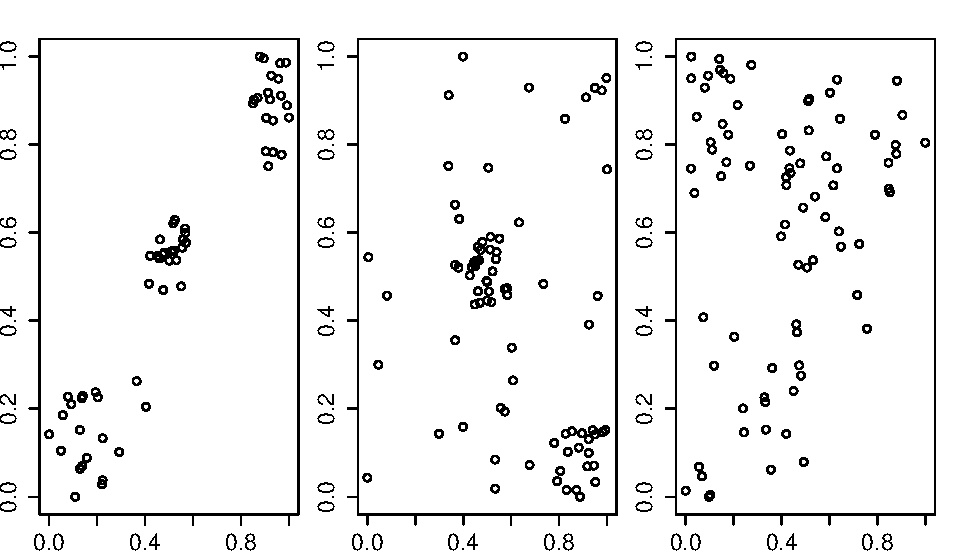
\includegraphics{clustering01.pdf}
\caption{Штучно сгенеровані набори даних}
\label{fig:clustering01}
\end{center}
\end{figure}

Кожен з наборів даних, що їх наведено на рис.~\ref{fig:clustering01} містить 80 спостережень з 2 ознаками (для наглядності) у кожному спостереженні. Тестові дані були сгенеровані таким чином, аби у першому наборі класи були чітко розподілені (crisp dataset), у другому наборі кластерні межі були дещо розмиті (fuzzy dataset), у третьому випадку класи сильно перетиналися (extra fuzzy dataset). Логічно припустити, що система, яка тестується, обере менше значення параметру фазифікації для першого датасету та більше для останнього, де межі класів спостережень є більш розмитими.

Спостереження надходили до нейро-фаззі мережі у послідовному режимі, вагові коефіцієнти нейронів були проініціалізовані використовуючи пакету модифікацію обраного алгоритму кластерування на датасеті з довільних двадцятьох спопрстережень відповідного набору даних (адже система, як і класичний fuzzy c-means, \hl{чутлива до ініціалзації)}. Локально оптимальні кількість кластерів та значення параметру фазифікації обумовлювалися максимальним середнім значенням рекурентних коефіцієнту розбиття PC \eqref{eq:reccurentPartitioningCoefficient} та Ксі-Бені індексу \eqref{eq:recurrentXieBeniIndex}: $\max{\frac{PC_j^{[m]} + 1 - XB_j^{[m]}}{2}}$ (у данному випадку використовувалося від'ємне значення Ксі-Бені індексу $1-XB\left(k\right)$, оскільки щоменше $XB_j^{[m]}$, толіпшим є розбиття даних на кластери). 

\begin{figure}
\begin{center}
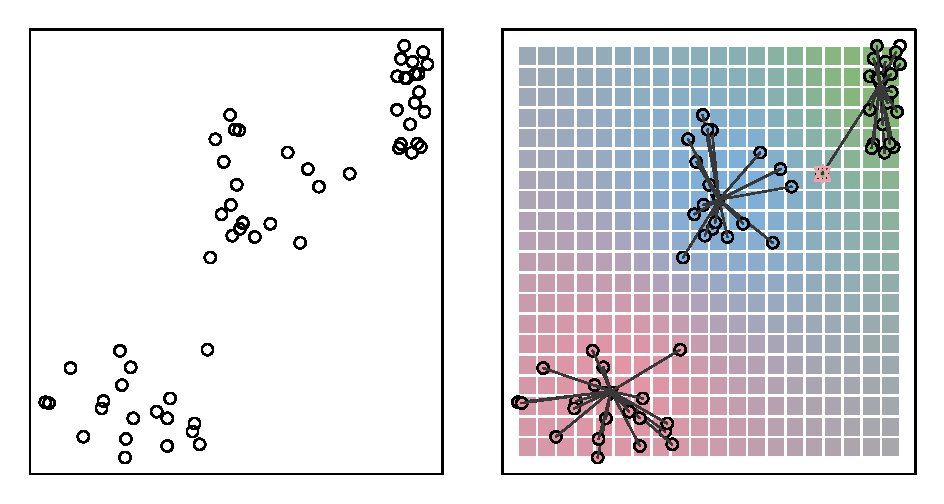
\includegraphics{clustering002.pdf}
\caption{Набір даних з чітко вираженими класами (Crisp dataset)}
\label{fig:clustering02}
\end{center}
\end{figure}

\begin{table}[ht]
\centering \small \begin{tabular}{rcccc}
\hline \multicolumn{4}{l}{Каскад 1 ($m=2$)}\\ \hline & Нейрон 1  & Нейрон 2 & Нейрон 3  & Нейрон 4 \\ &($\beta=2$) & ($\beta=3$) & ($\beta=4$) & ($\beta=5$) \\Коефіцієнт розбиття &
0.91758 & 0.7446 & 0.64787 & 0.59236 \\
Індекс Ксі-Бені &
0.052129 & 0.061034 & 0.092235 & 0.1294 \\
%——————————————————————————————————————————% 
\hline \multicolumn{4}{l}{Каскад 2 ($m=3$)}\\ \hline & Нейрон 1  & Нейрон 2 & Нейрон 3  & Нейрон 4 \\ &($\beta=2$) & ($\beta=3$) & ($\beta=4$) & ($\beta=5$) \\
Коефіцієнт розбиття &
0.92643 & 0.6609 & 0.50214 & 0.43305 \\
Індекс Ксі-Бені &
0.027232 & 0.06872 & 0.17281 & 0.26914 \\
%——————————————————————————————————————————% 
\hline \multicolumn{4}{l}{Каскад 3 ($m=4$)}\\ \hline & Нейрон 1  & Нейрон 2 & Нейрон 3  & Нейрон 4 \\ &($\beta=2$) & ($\beta=3$) & ($\beta=4$) & ($\beta=5$) \\
Коефіцієнт розбиття &
0.87218 & 0.5256 & 0.37605 & 0.31993 \\
Індекс Ксі-Бені &
0.15687 & 0.4153 & 0.84699 & 1.1765 \\
%——————————————————————————————————————————% 
\hline \multicolumn{4}{l}{Каскад 4 ($m=5$)}\\ \hline & Нейрон 1  & Нейрон 2 & Нейрон 3  & Нейрон 4 \\ &($\beta=2$) & ($\beta=3$) & ($\beta=4$) & ($\beta=5$) \\
Коефіцієнт розбиття &
0.73909 & 0.45445 & 0.32428 & 0.27063 \\
Індекс Ксі-Бені &
0.12985 & 0.30637 & 0.68584 & 1.0551 \\
\hline
\end{tabular}
\caption{Індекси валідності (датасет 1)}
\label{tabel:kysymys}
\end{table}

Для першого набору даних (crsip dataset), як і передбачалося, оптимальним виявися другий каскад ($m=3$) з трьома кластерами і нейроном-переможцем із найменшим значенням параметру фазифікацїї $\beta = 2$ (рис.~\ref{fig:clustering02}). Така конфігурація є оптимальною відповідно до обох використовуваних індексів валідності -- найменше значення Ксі-Бені індексу $XB_j^{[m]}$ та найбільший коефіцієнт розбиття $PC_j^{[m]}$: 

\begin{equation*}
\begin{aligned}
PC_1^{[2]}=&0.9009951,\\
XB_1^{[2]}=&0.03349166.
\end{aligned}
\end{equation*}
\medskip

Лише одне спостереження у цьому датасеті (його позначено багряним квадратом) не належить жодному кластерові з ступінем більшим від $0.6$. Індекси валідності нейронів системи наведені у таблиці \ref{table:kysymys}

\begin{figure}
\begin{center}
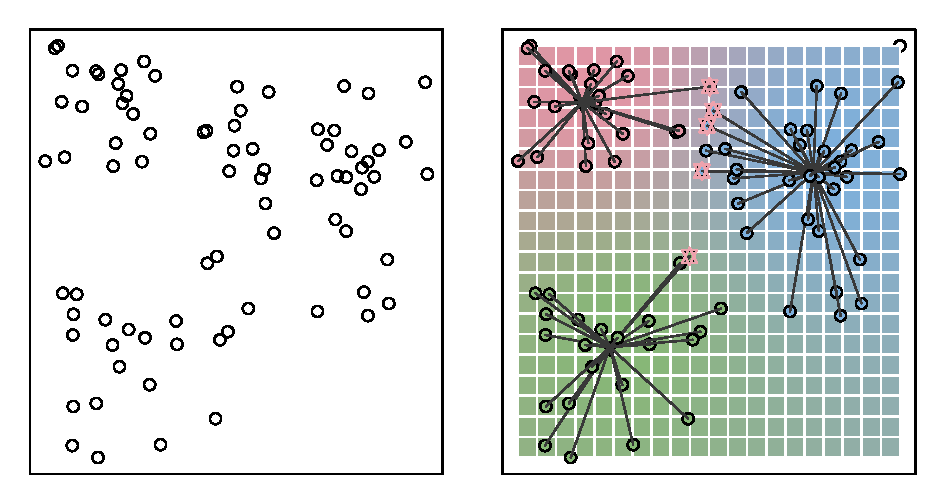
\includegraphics{clustering03.pdf}
\caption{Набір даних з нечіткими межами класів (fuzzy dataset)}
\label{fig:clustering03}
\end{center}
\end{figure}

Для набору даних з середньою вираженістю класів найліпшим виявився нейрон другого каскаду ($m=3$) і фаззифікатором $\beta=3$. Як показано на рис.~\ref{fig:clustering03}, декілька спостережень у центрі (позначені багряними квадратами) можна віднести до 2 кластерів з відносно високим ступінем належності, проте більшість спостережнь можна чітко розкластеризувати, що ілюструється високим значенням коефіцієнту розбиття, та дуже низьким Ксі-Бені індексом:

\begin{equation*}
\begin{aligned}
PC_2^{[2]}=&0.9727868,\\
XB_2^{[2]}=&0.009740618.
\end{aligned}
\end{equation*}
\medskip

\begin{figure}
\begin{center}
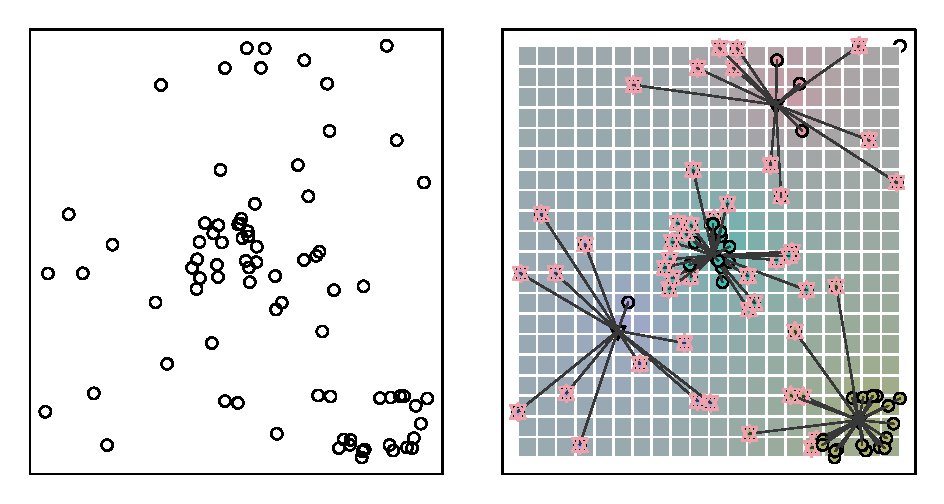
\includegraphics{clustering04.pdf}
\caption{Набір даних з класами, що перетинаються (extra fuzzy dataset)}
\label{fig:clustering04}
\end{center}
\end{figure}

Для набору з найменш чіткими межами класів, система обрала нейроном-переможцем вузол третього каскаду ($m=4$) з високим параметором фазифікації $\beta = 4$:

\begin{equation*}
\begin{aligned}
PC_3^{[3]}=&0.335525,\\
XB_3^{[3]}=&0.2128333.
\end{aligned}
\end{equation*}
\medskip

На рис.~\ref{fig:clustering04} спостереження, у яких ступінь належності до будь-якого кластеру не перевищує $0.6$ позначені багряними квадратами. Як і очікувалося,  для цього набору даних кількість таких спостережень значно вища від попередніх датасетів з більш компактними та <<чіткими>> класами.

Для наглядності у всіх наведених рисунках кольором позначені не тільки розкластеровані спостереження і центри кластерів, а й задній план (фон) малюнків, що дозволяє візуально визначити, до якого кластеру система віднесла б нові спостереження. Не дивно, тоді як для перших двох датасетів важко визначити домінуючий колір, оскільки кластери їх спостережень більш менш компактні та явно виражені, для останнього набору даних домінуючий колір сформований кольорами усіх кластерів, що ілюструє великий ступінь перекриття класів і, відповідно, високе значення оптимального параметру фазифікації $\beta$, що обрала система. 

Ця низка експериментів проілюструвала як важливо вірно визначати параметр фазифікації, оптимальне значення якого у випадку обробляння даних у послідовному режимі з високою вирогідністю змінюється у часі, а саме здатність визначати оптимальне значення цього параметру в онлайн режимі є відмінною особливістю попропонованої самонавчанної нейро-системи.

% Приклад посилання на таблицю
У табл.~\ref{tab:ellipse.hyperbola.parabola} наведені деякі
формули для еліпса, гіперболи і параболи.

% Приклад таблиці
\begin{table}[htbp]
\caption{Еліпс, гіпербола і парабола. Деякі формули}
\label{tab:ellipse.hyperbola.parabola}
\begin{tabularx}{\textwidth}{|X|c|c|c|}
\hline
                   & Еліпс                                    & Гіпербола                                & Парабола          \\
\hline
Канонічне рівняння & $\frac{x^2}{a^2}+\frac{y^2}{b^2}=1$      & $\frac{x^2}{a^2}-\frac{y^2}{b^2}=1$      & $y^2=2px$         \\
Ексцентриситет     & $\varepsilon=\sqrt{1-\frac{b^2}{a^2}}<1$ & $\varepsilon=\sqrt{1+\frac{b^2}{a^2}}>1$ & $\varepsilon=1$   \\
Фокуси             & $(a\varepsilon,0)$, $(-a\varepsilon,0)$  & $(a\varepsilon,0)$, $(-a\varepsilon,0)$  & $(\frac{p}{2},0)$ \\
\hline
\multicolumn{4}{|l|}{Корн~Г., Корн~Т. Справочник по математике. М., 1974. С.~72.} \\
\hline
\end{tabularx}
\end{table}


\bibliographystyle{ugost2008ns}
\bibliography{references}	

\end{document}